\documentclass[a4paper]{article}

\RequirePackage[undo-recent-deprecations]{expl3} %% Fix: latex3 problem with ebproof

\usepackage[pages=all, color=black, position={current page.south}, placement=bottom, scale=1, opacity=1, vshift=5mm]{background}
%% \SetBgContents{
%% 	\tt This work is shared under a \href{https://creativecommons.org/licenses/by-sa/4.0/}{CC BY-SA 4.0 license} unless otherwise noted
%% }      % copyright

\usepackage[margin=1in]{geometry} % full-width

% AMS Packages
\usepackage{amsmath}
\usepackage{amsthm}
\usepackage{amssymb}

% Unicode
\usepackage[utf8]{inputenc}
\usepackage{hyperref}
\hypersetup{
	unicode,
%	colorlinks,
%	breaklinks,
%	urlcolor=cyan, 
%	linkcolor=blue, 
	pdfauthor={Author One, Author Two, Author Three},
	pdftitle={A simple article template},
	pdfsubject={A simple article template},
	pdfkeywords={article, template, simple},
	pdfproducer={LaTeX},
	pdfcreator={pdflatex}
}

% Vietnamese
%\usepackage{vntex}

% Natbib
\usepackage[sort&compress,numbers,square]{natbib}
%\bibliographystyle{mplainnat}
\bibliographystyle{plain}
  
% Theorem, Lemma, etc
\theoremstyle{plain}
\newtheorem{theorem}{Theorem}
\newtheorem{corollary}[theorem]{Corollary}
\newtheorem{lemma}[theorem]{Lemma}
\newtheorem{claim}{Claim}[theorem]
\newtheorem{axiom}[theorem]{Axiom}
\newtheorem{conjecture}[theorem]{Conjecture}
\newtheorem{fact}[theorem]{Fact}
\newtheorem{hypothesis}[theorem]{Hypothesis}
\newtheorem{assumption}[theorem]{Assumption}
\newtheorem{proposition}[theorem]{Proposition}
\newtheorem{criterion}[theorem]{Criterion}
\theoremstyle{definition}
\newtheorem{definition}[theorem]{Definition}
\newtheorem{example}[theorem]{Example}
\newtheorem{remark}[theorem]{Remark}
\newtheorem{problem}[theorem]{Problem}
\newtheorem{principle}[theorem]{Principle}

%%% ebproof column width
\newcommand{\rulewidth}{.8\linewidth}
\newcommand{\ruleverticalsephalf}{0.25cm}
\newcommand{\ruleverticalsep}{0.5cm}

\usepackage{graphicx, color}
\graphicspath{{fig/}}

%\usepackage[linesnumbered,ruled,vlined,commentsnumbered]{algorithm2e} % use algorithm2e for typesetting algorithms
\usepackage{algorithm, algpseudocode} % use algorithm and algorithmicx for typesetting algorithms
\usepackage{mathrsfs} % for \mathscr command

\usepackage{lipsum}

%%% RPC Calculi related commands %%%

%%
\usepackage{listings}
\lstset
{
    basicstyle=\footnotesize\ttfamily,
    numbers=left,
    stepnumber=1,
    frame=single,
}
\usepackage{ebproof}
\usepackage{multicol}
\usepackage{xspace}
\usepackage{stmaryrd} % \llbracket \rrbracket

%% Macros for General Inference Rules
\newcommand{\rpc}{$\lambda_{rpc}$\xspace}
\newcommand{\typedrpc}{$\lambda_{rpc}^{typed}$\xspace}
\newcommand{\polyrpc}{$\lambda_{rpc}^{\forall}$\xspace}
\newcommand{\linksrpc}{$\lambda_{rpc}^{Links}$\xspace}
\newcommand{\kindedpolyrpc}{$\lambda_{rpc}^{\forall,k}$\xspace}

\newcommand{\stateencrpc}{$\lambda_{rpc}^{enc}$\xspace}
\newcommand{\statefulrpc}{$\lambda_{rpc}^{state}$\xspace}

\newcommand{\cs}{$\lambda_{cs}$\xspace}
\newcommand{\polycs}{$\lambda_{cs}^{\forall}$\xspace}
\newcommand{\stateenccs}{$\lambda_{cs}^{enc}$\xspace}
\newcommand{\statefulcs}{$\lambda_{cs}^{state}$\xpace}

\newcommand{\client}{\textbf{c}}
\newcommand{\server}{\textbf{s}}
\newcommand{\clientserver}{\textbf{cs}}

\newcommand{\statickind}{sta}
\newcommand{\dynamickind}{dyn}

\newcommand{\evalRPC}[3]{#1\Downarrow_{#2}#3}
\newcommand{\evalRPCC}[2]{#1\Downarrow_{\client}#2}
\newcommand{\evalRPCS}[2]{#1\Downarrow_{\server}#2}
\newcommand{\lamL}[3]{\lambda^{#1}#2.#3}
\newcommand{\appL}[3]{#1{\ }^{#2}#3}
\newcommand{\subst}[2]{\{#1/#2\}}
\newcommand{\llet}[3]{\textsf{let} \ #1 = #2 \ \textsf{in} \ #3}
\newcommand{\ldokeyword}{\textsf{do}}
\newcommand{\ldo}[3]{\textsf{do} \ #1 \leftarrow #2 \ \textsf{in} \ #3}
\newcommand{\ldovoid}[2]{\textsf{do} \ #1 \ \textsf{in} \ #2}
\newcommand{\lunit}[1]{\textsf{unit} \ #1}

\newcommand{\textsfGen}{\textsf{gen}}
\newcommand{\gen}[3]{\textsfGen(#1,#2,#3)}

\newcommand{\textsfReq}{\textsf{req}}
\newcommand{\req}[2]{\textsfReq(#1,#2)}

\newcommand{\textsfCall}{\textsf{call}}
\newcommand{\call}[2]{\textsfCall(#1,#2)}

\newcommand{\textsfRet}{\textsf{ret}}
\newcommand{\ret}[1]{\textsfRet(#1)}

\newcommand{\textsfCase}{\textsf{case}}
\newcommand{\textsfOf}{\textsf{of}}
\newcommand{\case}[2]{\textsfCase ~ #1 ~\textsfOf ~ #2}

\newcommand{\fun}{\rightarrow}
\newcommand{\funL}[1]{\xrightarrow{#1}}
\newcommand{\funLC}[2]{\xrightarrow[#2]{#1}}
\newcommand{\tyenv}{\Gamma}
\newcommand{\tyenvExt}[2]{\Gamma,#1:#2}
\newcommand{\tyenvExtWith}[1]{\Gamma,#1}
\newcommand{\varenv}{\Delta}
\newcommand{\varenvExt}[1]{\Delta,#1}
%\newcommand{\typing}[4]{#1\rhd_{#2} #3 : #4}
\newcommand{\typing}[4]{#1\vdash_{#2} #3 : #4}
\newcommand{\kinding}[3]{#1\vdash #2 : #3}
\newcommand{\funtyping}[5]{#1\vdash #4 : #5}     % ;#2, #3
\newcommand{\codetyping}[4]{#1\vdash_{code} #3 : #4}  % _{#2}
\newcommand{\polytyping}[5]{#1;#2\vdash_{#3} #4 : #5}
\newcommand{\conftyping}[2]{\vdash #1 : #2}
\newcommand{\stacktyping}[3]{\vdash_{#1} #2 : #3}
\newcommand{\fvtyping}[2]{#1\vdash #2}

\newcommand{\typingBlack}[4]{#1\blacktriangleright_{#2} #3 : #4}

\newcommand{\loceta}[2]{{#1}\rightsquigarrow{#2}}

\newcommand{\enc}{\textsf{enc}}
\newcommand{\evalStateEncRPCC}[2]{$#1\Downarrow_{\client}^{\enc}#2$}
\newcommand{\evalStateEncRPCS}[3]{$#1;#2\Downarrow_{\server}^{\enc}#3$}

\newcommand{\sta}{\textsf{state}}
\newcommand{\evalStatefulRPCC}[3]{\evalStatefulRPC{#1}{#2}{\client}{#3}}
\newcommand{\evalStatefulRPCS}[3]{\evalStatefulRPC{#1}{#2}{\server}{#3}}
\newcommand{\evalStatefulRPC}[4]{${#1};{#2}\Downarrow_{#3}^{\sta}{#4}$}

\newcommand{\deep}{\textsf{deep}}
\newcommand{\evalDeeplyStatefulRPCC}[3]{\evalDeeplyStatefulRPC{#1}{#2}{\client}{#3}}
\newcommand{\evalDeeplyStatefulRPCS}[3]{\evalDeeplyStatefulRPC{#1}{#2}{\server}{#3}}
\newcommand{\evalDeeplyStatefulRPC}[4]{${#1};{#2}\Downarrow_{#3}^{\deep}{#4}$}

\newcommand{\IdK}{\textsf{Id}}
\newcommand{\FunK}[3]{\textsf{Fun} \ #2 \ #3}
\newcommand{\AppK}[3]{\textsf{App} \ #2 \ #3}
%\newcommand{\FunK}[3]{\textsf{Fun}^{#1} \ #2 \ #3}
%\newcommand{\AppK}[3]{\textsf{App}^{#1} \ #2 \ #3}

\newcommand{\reify}[1]{\ulcorner #1 \urcorner}

\newcommand{\RightarrowEnc}{\Rightarrow^{enc}}
\newcommand{\RightarrowEncStar}{\Rightarrow^{enc*}}
\newcommand{\RightarrowEncPlus}{\Rightarrow^{enc+}}

\newcommand{\runStateEncRPC}[2]{$#1 \RightarrowEnc #2$}
\newcommand{\runStateEncRPCStar}[2]{$#1 \RightarrowEncStar #2$}
\newcommand{\runStateEncRPCPlus}[2]{$#1 \RightarrowEncPlus #2$}

\newcommand{\runStateEncCS}[2]{$#1 \Rightarrow^{enc} #2$}
\newcommand{\runStateEncCSStar}[2]{$#1 \Rightarrow^{enc*} #2$}

\newcommand{\runStatefulRPC}[2]{$#1 \Rightarrow^{state} #2$}
\newcommand{\runStatefulRPCStar}[2]{$#1 \Rightarrow^{state*} #2$}

\newcommand{\runStatefulCS}[2]{$#1 \Rightarrow^{state} #2$}
\newcommand{\runStatefulCSStar}[2]{$#1 \Rightarrow^{state*} #2$}

\newcommand{\emp}{\epsilon}
\newcommand{\substzsxs}{\{\bar{v}/\bar{z},\overline{w}/\bar{x} \}}
\newcommand{\substxs}{\{\overline{w}/\bar{x} \}}

\newcommand{\substZsXs}{\{\overline{V}/\bar{z},\overline{W}/\bar{x} \}}
\newcommand{\substXs}{\{\overline{W}/\bar{x} \}}

\newcommand{\LetK}[2]{\textsf{ctx}\ #1 \ #2}
%\newcommand{\LetK}[2]{(#1,#2)}
\newcommand{\opt}[1]{#1_{opt}}

\newcommand{\overlineK}{\overline{K}}
\newcommand{\overlinePi}{\overline{\Pi}}
\newcommand{\overlineDelta}{\overline{\Delta}}

%\newcommand{\comp}[1]{\rightsquigarrow_{#1}}
%\newcommand{\comps}{\rightsquigarrow_{\server}}
%\newcommand{\compc}{\rightsquigarrow_{\client}}
% \newcommand{\ccomp}[1]{\mathcal{C}[\![#1]\!]}
\newcommand{\ccomp}[1]{\mathcal{C}\llbracket#1\rrbracket}
%\newcommand{\scomp}[1]{S[\![#1]\!]}
% \newcommand{\vcomp}[1]{\mathcal{V}[\![#1]\!]}
\newcommand{\vcomp}[1]{\mathcal{V}\llbracket#1\rrbracket}
%\newcommand{\cconv}[1]{CC[\![#1]\!]}
%\newcommand{\cconvprg}[1]{CC_{prg}[\![#1]\!]}
\newcommand{\typeinf}[1]{G[\![#1]\!]}

% \newcommand{\ecomp}[1]{[\![#1]\!]}
\newcommand{\ecomp}[1]{\llbracket#1\rrbracket}

\newcommand{\linkstycomp}[2]{\llbracket#1\rrbracket_{#2}}
\newcommand{\adjcomp}[4]{#1:#2 \Rightarrow #3:#4}
\newcommand{\judgcomp}[2]{\llbracket#1\rrbracket_{#2}}

\newcommand{\loctycomp}[1]{L\llbracket#1\rrbracket}
\newcommand{\polytycomp}[1]{T\llbracket#1\rrbracket}

\newcommand{\anncomp}[1]{Ann\llbracket#1\rrbracket}
\newcommand{\loctmcomp}[1]{\llbracket#1\rrbracket}


\newcommand{\FUNS}{\Phi}
\newcommand{\funstore}{\FUNS}
\newcommand{\funtype}{\funstore_{type}}
\newcommand{\funcode}{\funstore}
\newcommand{\fv}[1]{\textsf{fv}(#1)}
\newcommand{\dom}[1]{\textsf{dom}(#1)}
\newcommand{\clo}[2]{clo({#1},{#2})}
\newcommand{\cloty}[1]{Clo(#1)}
\newcommand{\valty}[1]{relocatable(#1)}

\newcommand{\Loc}{Loc}

\newcommand{\sessionNothing}{\makebox[0.3cm][c]{\scriptsize $nothing$}}
\newcommand{\sessionSomething}{\makebox[0.3cm][c]{\scriptsize $session$}}
\newcommand{\sessionOption}{\makebox[0.3cm][c]{\scriptsize $optSession$}}

\newcommand{\mono}[1]{[\![#1]\!]}

\newcommand{\optrpc}[1]{\mathcal{O}[\![#1]\!]}

\newcommand{\resolve}[2]{\{\!\{#1\}\!\}^{#2}}

\newcommand{\stack}{\Delta}
\newcommand{\emptystack}{\epsilon}

\newcommand{\conf}{\Sigma}
\newcommand{\confcs}[2]{\langle #1 | #2 \rangle}
\newcommand{\stackcsWith}[2]{ #1  |  #2 }
\newcommand{\stackcs}{\stackcsWith{ \stack_\client }{ \stack_\server }}
\newcommand{\confuntyped}{\sigma}

\newcommand{\run}{\longrightarrow}
\newcommand{\runequiv}{\Longrightarrow}
\newcommand{\structeqv}{\equiv}

\newcommand{\loctyvars}{\overline{l} \ \overline{\alpha}}
\newcommand{\loctys}{\overline{\Loc}\ \overline{A}}

\newcommand{\CloCodeType}{Ty}
\newcommand{\CloCode}{Code}
\newcommand{\OpenCode}{OpenCode}

%%%%%%%%%%%%%%%%%%%%%%%%%%%%%%%%%%%%



% Author info
\title{On Recovering Static Location Contexts in Links\\(A progress report)}
\author{Kwanghoon Choi}
%\author{Author One$^1$\thanks{Author One was partially supported by Grant XXX} \and Author Two$^2$ \and Author Three$^1$}

\date{
  Chonnam National University, Gwangju, Republic of Korea
  \\ \texttt{kwanghoon.choi@jnu.ac.kr}\\[2ex]%
	%% $^1$Organization 1 \\ \texttt{\{auth1, auth3\}@org1.edu}\\%
	%% $^2$Organization 2 \\ \texttt{auth3@inst2.edu}\\[2ex]%
%	\today
}

\begin{document}

\maketitle
	
\begin{abstract}
%
This progress report describes an attempt to recover static location
contexts in the Links-RPC calculus, which represents the RPC aspect of
Links, by compiling to the polymorphic RPC calculus and back to
itself.
%  
Currently, the proposed idea is limited to the rank-1 subset of the
Links-RPC calculus.
%
The limitation is caused by a technical problem involving polymorphic
constructs in the adjustment of locations to resolve the location
discrepancies resulting from our heuristic type compilation.
%
We will continue to study to extend the applicability to the whole
calculus by solving this problem.

\noindent\textbf{Keywords:} Location inference, Links, RPC calculus
\end{abstract}

%\tableofcontents
	
\section{Introduction}
\label{sec:intro}

A motivation is this.
%
The feature of location types would be good for providing multi-tier
programming languages like Links static location contexts useful for
optimization of local computation and statically checking location
inconsistencies.
%
However, a naive integration of this feature in Links should be
challenging because several advanced features have been developed and
they might require to be changed in a significant way.
%
As an alternative to this direction, we study a way to recover static
location contexts in Links in the hope of no change or, if there is
any, minimal changes that do not impact the language system of Links.



Figure~\ref{fig:addingstaticlocationcontexts}.
\begin{figure}[ht]
        \centering
        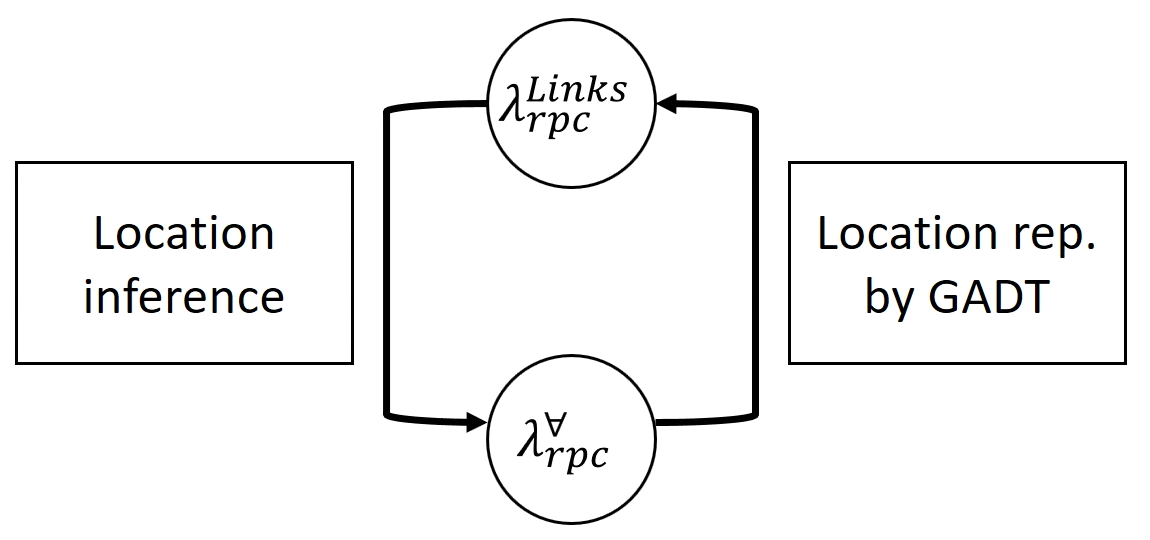
\includegraphics[width=0.6\textwidth]{linksrpc.png}
        \caption{Recovering static location contexts by compiling
          to the polymorphic RPC calculus and back}
        \label{fig:addingstaticlocationcontexts}
\end{figure}



%\lipsum[2]
	
%% \subsection{Preliminaries}
%% \label{sec:pre}
	
%% \lipsum[3]
	
%% \subsection{Previous Results}
%% \label{sec:prev-results}
	
%% Null graphs are discussed in \cite{HararyR74}
%% The concept of ``internally stable set'' was used in \cite{Berge57, Berge58}.
	
%% \begin{theorem}
%% 	\label{thrm:1}
%% 	\lipsum[4]
%% \end{theorem}
%% \begin{proof}
%% 	content...
%% \end{proof}

%% \begin{corollary}
%% \label{cor:1}
	
%% \lipsum[5]
%% \end{corollary}

%% Unordered List (taken from Overleaf)
%% \begin{itemize}
%% 	\item The individual entries are indicated with a black dot, a so-called bullet.
%% 	\item The text in the entries may be of any length.
%% \end{itemize}

%% Ordered List (taken from Overleaf)
%% \begin{enumerate}
%% 	\item The labels consists of sequential numbers.
%% 	\item The numbers starts at 1 with every call to the enumerate environment.
%% \end{enumerate}

%% \begin{table}[ht]
%% 	\centering
%% 	\begin{tabular}{|c|c|}
%% 		\hline
%% 		\textbf{Odd} & \textbf{Even} \\
%% 		\hline\hline
%% 		One & Two \\
%% 		\hline
%% 		Three & Four \\
%% 		\hline
%% 	\end{tabular}
%% 	\caption{This is a table}
%% 	\label{tbl:1}
%% \end{table}

%% Table~\ref*{tbl:1} is an example of a table.
	
\section{A Links-RPC Calculus}
\label{sec:linksrpc}

This section describes a RPC calculus that extends the RPC calculus
\cite{Cooper:2009:RC:1599410.1599439} with unannotated
$\lambda$-abstractions whose location is not specified.
%
The extended RPC calculus intends to capture the RPC feature of the
Links programming language \cite{Cooper:2006:LWP:1777707.1777724} in a
simple way.
%
For our setting, the calculus is also extended with type abstractions
and applications.
%
Let us call it a Links-RPC calculus, \linksrpc.


\begin{figure}[h]
\centering  
\begin{tabular}{ l  l  r  c  l }
\multicolumn{5}{l}{\textbf{Syntax}} \\
 & Location & $a,b$   & $::=$ & $\client \ \ | \  \  \server$ \\
 &          & $?a$    & $::=$  & $a  \ \ |  \ \ (unknown) $ \\
 & Term     & $L,M,N$ & $::=$  & $V  \ | \  L \ M  \ | \  M[A]  \ | \  (L,M)  \ |  \ \pi_i(M)$ \\
 & Value & $V,W$ & $::=$ & $x  \ \ |  \ \ \lambda^{?a} x.M  \ \ |  \ \ \Lambda\alpha.V  \ \ |  \ \ (V,W)$
\\[\ruleverticalsep]
\multicolumn{5}{l}{\textbf{Types}} \\
& Type & $A,B,C$ & $::=$
& $base  \ \ | \ \  A \rightarrow B  \ \ | \ \  \alpha  \ \ | \ \  A \times B  \ \ | \ \  \forall\alpha.A$
\end{tabular}
\caption{The Links-RPC calculus \linksrpc}
\label{fig:linksrpc}
\end{figure}

The terms and types of the Links-RPC calculus are shown in
Figure~\ref{fig:linksrpc}.
%
In the calculus, it is not mandatory to annotate locations to
$\lambda$ abstractions. This is for programmers' convenience.
%
$?a$ means that every annotation is either a location constant $a$ or
unknown.
%
Regardless of the presence of location annotations, function types are
$A \rightarrow B$ with no locations in a type-level.
%
No notion of location variables is available in the calculus, and so
there are no location abstractions nor applications.
%
Other than these differences, the terms and types are almost the same
as those for the polymorphic RPC calculus, which
is in the appendix for reference.
%


The semantics for \linksrpc includes an evaluation rule for
unannotated $\lambda$-abstractions, which once was proposed by the
original RPC calculus \cite{Cooper:2009:RC:1599410.1599439}, that
evaluate to $\lambda$-abstractions annotated with the location of
evaluation as
\[
\begin{prooftree}
  \infer[left label=(Unknown-Abs)]0{ \evalRPC{\lamL{}{x}{M}}{a}{\lamL{a}{x}{M} }}
\end{prooftree}
\]
%

The typing rules are actually the same as for the System-F calculus
except the appearance of annotated $\lambda$-abstractions whose
locations are disregarded by types.
%
\[
\begin{prooftree}
  \hypo{ \typing{\tyenvExt{x}{A}}{}{M}{B} }
  \infer[left label=(T-?a-Abs)]1{ \typing{\tyenv}{}{\lamL{?a}{x}{M}}{A \rightarrow B} }
\end{prooftree}
\]

For brevity, we omit writing the full definitions of the semantics and
the typing rules for \linksrpc.

\section{Compiling \linksrpc into \polyrpc}
\label{sec:translationtopolyrpc}

The purpose of compiling the Links-RPC calculus into the polymorphic
RPC calculus is to recover location information during the evaluation of
\linksrpc terms and to express it by located types of \polyrpc explicitly.
%
Such statically recovered location information would be made use of
later for transformations and optimizations, such as avoiding
unnecessary location checking at runtime for solely local computation.
%
Basically, this compilation would translate normal function types
$A_1 \rightarrow A_2$ into located function types $A_1' \funL{\Loc}
A_2'$ for some $A_i$s.
%
Then where do locations, such as $\Loc$, come from?
%
Generally, they are nowhere in the Links-RPC terms and types.
%
Therefore, a heuristic should be introduced to recover location
information lack in the terms and types.


A heuristic approach is to view \linksrpc types $A$ as \polyrpc types $B$ where
%
\begin{itemize}
  \item the {\it skeleton} of $B$ obtained from erasing all locations
    from it is the same as $A$, and
  \item all the erased locations are assumed to be the same as a given
    location $\Loc$.
\end{itemize}
%
For example, the type of a client map function, $(Int \rightarrow Int)
\rightarrow [Int] \rightarrow [Int]$, can be viewed as $(Int \funL{\client}
Int) \funL{\client} [Int] \funL{\client} [Int]$.
%
As is seen, not only the two function types on the spine get client
locations but the argument function type is also annotated with it.


%
This idea can be formulated as a type translation $\linkstycomp{A}{\Loc} = B$:

\begin{figure}[h]
\centering
\begin{tabular}{l l l l l l l l l l l l l l}
$\linkstycomp{\alpha}{\Loc}$ & $=$ & $\alpha$
&
$\linkstycomp{A \funL{} B}{\Loc}$ & $=$ & $\linkstycomp{A}{\Loc} \funL{Loc} \linkstycomp{B}{\Loc}$
\\
$\linkstycomp{base}{\Loc}$ & $=$ & $base$
&
$\linkstycomp{A\times B}{\Loc}$ & $=$ & $\linkstycomp{A}{\Loc}\times \linkstycomp{B}{\Loc}$
&
$\linkstycomp{\forall\alpha.A}{\Loc}$ & $=$ & $\forall\alpha.\linkstycomp{A}{\Loc}$
\\
\end{tabular}
\caption{A type compilation of \linksrpc into \polyrpc}
\label{fig:typecompilation}
\end{figure}

Note that the explained client map function type in \polyrpc is
obtained from $\linkstycomp{(Int \rightarrow Int) \rightarrow [Int] \rightarrow
  [Int]}{\client}$ by extending it over list types as
$\linkstycomp{[A]}{\Loc} = [ \linkstycomp{A}{\Loc} ]$ in a straightforward way.

Obviously, this heurisitc is not always satisfactory.
%
For example, $map \ f \ list$ is legitimate in \linksrpc even when
$map$ of the client map function type takes a function of type $Int
\funL{\client} Int$ but $f$ of type $Int \funL{\server} Int$ is given
as an argument in \polyrpc.
%
This is because \linksrpc can deal with this discrepancy by runtime
location checking.
%
However, there should be some adjustments to locations in compiled
types and terms.

A type-directed location adjustment is formulated as the following
form of judgments:
\[
\adjcomp{M}{A}{M'}{A'}
\]
From a term $M$ of type $A$, a new adjusted term $M'$ is derived under
the guidance of another type $A'$ having the same skeleton as but
possibly locatational discrepancies with $A$.
%
For example,
\[
\adjcomp{f}{Int \funL{\server} Int \ }{\ (\lamL{\client}{x}{f
    \ x})}{Int \funL{\client} Int}
\]
where given the three inputs, the adjusted client function
$\lamL{\client}{x}{f \ x}$ is derived.
%
Then the adjusted function could be fed into the client map function
as its first argument in \polyrpc.

A type-directed location adjustment to terms is formulated as
Figure~\ref{fig:locationadjustment}.
%
The rules are defined in terms of type structure, actually doing the
eta conversion for function, pair, polymorphic, polymorphic location
types of given terms.
%
By the conversion, they will adjust all discrepant locations of two
function types to produce new terms of the adjusted types.
%


\begin{figure}[h]
\centering
\begin{tabular}{p{\linewidth}}
  {
    \begin{prooftree}
      \hypo{  }
      \infer1{ \adjcomp{M}{A}{M}{A} }
    \end{prooftree}
    \ \ \ \ \
    \begin{prooftree}
      \hypo{ \adjcomp{x}{C}{N}{A} \ \ \ \adjcomp{M \ N}{B}{M'}{D} }
      \infer1{ \adjcomp{M}{A\funL{\Loc_1}B}{\lamL{\Loc_2}{x}{M'}}{C\funL{\Loc_2}D} }
    \end{prooftree}
    \ \ \ \ \
    \begin{prooftree}
      \hypo{ \adjcomp{\pi_i{M}}{A_i}{M_i'}{A_i'} \ \ \ (i=1,2) }
      \infer1{ \adjcomp{M}{A_1 \times A_2}{(M_1,M_2)}{A_1'\times A_2'} }
    \end{prooftree}
  }
\\[\ruleverticalsep]
  {
    \begin{prooftree}
      \hypo{ \adjcomp{M[\alpha]}{A}{M'}{B} }
      \infer1{ \adjcomp{M}{\forall\alpha.A}{\Lambda\alpha.M'}{\forall\alpha.B} }
    \end{prooftree}
    \ \ \ \ \
    \begin{prooftree}
      \hypo{ \adjcomp{M[l]}{A}{M'}{B} }
      \infer1{ \adjcomp{M}{\forall l.A}{\Lambda l.M'}{\forall l.B} }
    \end{prooftree}
  }
\end{tabular}
\caption{A type-directed location adjustment to terms}
\label{fig:locationadjustment}
\end{figure}

Using the rules, one can derive the example adjustment judgment for
given $f$, the server function type, and the client function,
producing the adjusted term, $\lamL{\client}{x}{f \ x}$.

Based on the heuristic type compilation with the type-directed
location adjustment, we can define the compilation rules of \linksrpc
into \polyrpc as shown in Figure~\ref{fig:compilationoflinksrpc}.

\begin{figure}[h]
\centering
\begin{tabular}{l c p{\rulewidth}}
  $\judgcomp{ \typing{\tyenv}{}{x}{A} }{\Delta,\Loc}$ & $=$
  & {
      \begin{prooftree}
        \hypo{ x:B \in \Delta }
        \infer1{ \typing{\Delta}{\Loc}{x}{B} }
      \end{prooftree}
    }
  \\[\ruleverticalsep]
%  
  $\judgcomp{ \typing{\tyenv}{}{\lamL{a}{x}{M}}{A \rightarrow B} }{\Delta,\Loc}$ & $=$
  & let $\typing{\Delta,x:\linkstycomp{A}{a}}{a}{M'}{D}$
    \ = \ $\judgcomp{ \typing{\tyenvExt{x}{A}}{}{M}{B} }{(\Delta,x:\linkstycomp{A}{a}),a}$
  \\[\ruleverticalsephalf]
  &
  & $\typing{\Delta}{\Loc}{\lamL{a}{x}{M'}}{\linkstycomp{A}{a} \funL{a} D}$
  \\[\ruleverticalsep]
%  
  $\judgcomp{ \typing{\tyenv}{}{\lamL{}{x}{M}}{A \rightarrow B} }{\Delta,\Loc}$ & $=$
  & let $l$ be fresh
  \\
  &
  & let $\typing{\Delta,l,x:\linkstycomp{A}{l}}{l}{M'}{D}$
    \ = \ $\judgcomp{ \typing{\tyenvExt{x}{A}}{}{M}{B} }{(\Delta,l,x:\linkstycomp{A}{l}),l}$
  \\[\ruleverticalsephalf]
  &
  & {
      \begin{prooftree}
        \hypo{
          \begin{prooftree}
            \hypo{ \typing{\Delta,l}{\Loc}{\lamL{l}{x}{M'} }{ \linkstycomp{A}{l}\funL{l}D } }
            \infer1{ \typing{\Delta}{\Loc}{\Lambda l.\lamL{l}{x}{M'} }{ \forall l.(\linkstycomp{A}{l}\funL{l}D) } }
          \end{prooftree}
        }
        \infer1{ \typing{\Delta}{\Loc}{(\Lambda l.\lamL{l}{x}{M'})[\Loc] }{ (\linkstycomp{A}{l}\funL{l}D)\subst{\Loc}{l}} }
      \end{prooftree}
    }
  
  \\[\ruleverticalsephalf]
%  
  $\judgcomp{ \typing{\tyenv}{}{M \ N }{B} }{\Delta,\Loc}$ & $=$
  & let $\typing{\Delta}{\Loc}{M'}{C \funL{\Loc'} D}$
    \ = \ $\judgcomp{ \typing{\tyenv}{}{M}{A \rightarrow B} }{\Delta,\Loc}$
  \\[\ruleverticalsephalf]
  &
  & let $\typing{\Delta}{\Loc}{N_0'}{C_0}$
    \ = \ $\judgcomp{ \typing{\tyenv}{}{N}{A} }{\Delta,\Loc}$
  \\[\ruleverticalsephalf]
  &
  & let $\adjcomp{N_0'}{C_0}{N'}{C}$
  \\[\ruleverticalsephalf]
  &
  & $\typing{\Delta}{\Loc}{M' \ N'}{D}$
  \\[\ruleverticalsep]
%  
  $\judgcomp{ \typing{\tyenv}{}{(M_1,M_2)}{A_1\times A_2} }{\Delta,\Loc}$ & $=$
  & let $\typing{\Delta}{\Loc}{M_i'}{A_i'}$
    \ = \ $\judgcomp{ \typing{\tyenv}{}{M_i}{A_i} }{\Delta,\Loc}$ for $i=1,2$
  \\[\ruleverticalsephalf]
  &
  & $\typing{\Delta}{\Loc}{(M_1',M_2')}{(A_1' \times A_2')}$
  \\[\ruleverticalsep]
%  
  $\judgcomp{ \typing{\tyenv}{}{\pi_i M}{A_i} }{\Delta,\Loc}$ & $=$
  & let $\typing{\Delta}{\Loc}{M'}{A_1' \times A_2'}$
    \ = \ $\judgcomp{ \typing{\tyenv}{}{M}{A_1\times A_2} }{\Delta,\Loc}$
  \\[\ruleverticalsephalf]
  &
  & $\typing{\Delta}{\Loc}{\pi_i \ M'}{A_i'}$
  \\[\ruleverticalsep]
%  
  $\judgcomp{ \typing{\tyenv}{}{\Lambda\alpha.V}{\forall\alpha.A} }{\Delta,\Loc}$ & $=$
  & let $\typing{\Delta,\alpha}{\Loc}{V'}{A'}$
    \ = \ $\judgcomp{ \typing{\tyenv,\alpha}{}{V}{A} }{(\Delta,\alpha),\Loc}$
  \\[\ruleverticalsephalf]
  &
  & $\typing{\Delta}{\Loc}{\Lambda\alpha.V'}{\forall\alpha.A'}$
  \\[\ruleverticalsep]
%  
  $\judgcomp{ \typing{\tyenv}{}{M \ [B]}{A\subst{B}{\alpha}} }{\Delta,\Loc}$ & $=$
  & let $\typing{\Delta}{\Loc}{M'}{\forall\alpha.C}$
    \ = \ $\judgcomp{ \typing{\tyenv}{}{M}{\forall\alpha.A} }{\Delta,\Loc}$
  \\[\ruleverticalsephalf]
  &
  & $\typing{\Delta}{\Loc}{M'[ \ \linkstycomp{B}{\Loc} \ ]}{C\subst{ \linkstycomp{B}{\Loc} }{\alpha}}$
  \\[\ruleverticalsep]
\end{tabular}
\caption{A compilation of \linksrpc into \polyrpc}
\label{fig:compilationoflinksrpc}
\end{figure}


%
Basically, the compilation rules forms a transformation
$\judgcomp{\mathcal{D}}{\Delta,\Loc}=\mathcal{D'}$ of typing derivations
$\mathcal{D}$ in \linksrpc into those $\mathcal{D'}$ in \polyrpc.
%
Additionally, as contextual information in \polyrpc, the
compilation method is defined to take a type environment $\Delta$ and a
location $\Loc$.
%
The type environment $\Delta$ provides how types for free variables in
\linksrpc are heuristically compiled depending on locational contexts.
%
The location $\Loc$ informs where terms being compiled are.


%
One of the most important compilation rules is for $\lambda$-applications $M
\ N$.
%
After $M$ and $N$ are compiled into $M'$ and $N_0'$, the compiled
argument term is adjusted to the argument type of the compiled
functional term.

%
Unannotated $\lambda$-abstractions are compiled into location
abstractions that are subsequently instantiated with the location of
the $\lambda$-abstractions.

%
Note that compiling $\lamL{?a}{x}{M}$ of type $A \rightarrow B$ at a
locational context $\Loc$ extends the current type environment with a
type binding of $x$ and a heuristically compiled argument type, that
is, $\linkstycomp{A}{a}$ or $\linkstycomp{A}{l}$ for some fresh location
variable.

\subsection{Problem: Violating Syntactic Restriction on Polymorphism}

%
We have a problem in the formulation of the compilation of \linksrpc
into \polyrpc.
%
Recall that type and location abstractions are defined in the form as
$\Lambda\alpha.V$ and $\Lambda l.V$ where the bodies are in the form
of values.
%
The compilation of arbitrary ranked \linksrpc terms could produce
\polyrpc terms that violate this syntactic restriction.
%
For those \linksrpc terms of polymorphic types under the rank-1
polymorphism, often called the Hindley-Milner style polymorphism, the
proposed compilation rules will always produce legitimate terms
keeping the polymorphic restriction in syntax.

%
The cause of the problem is that the eta-conversion of type and
location abstractions leads to type and location applications in their
bodies.
%
Let us explain the cause by example.
%
It is legitimate to have an adjustment as
\[
\adjcomp{\Lambda\alpha.(\lamL{\client}{x}{x}, 42)}
        {\forall\alpha.(\alpha\funL{\client}\alpha\times Int) \ \ }
        {\ \ \Lambda\alpha.(\lamL{\server}{x}{x}, 42)}
        {\forall\alpha.(\alpha\funL{\server}\alpha\times Int)}
\]
when the body of the type abstraction is known.
%
Otherwise, it seems only to have
\[
\adjcomp{f}
        {\forall\alpha.(\alpha\funL{\client}\alpha\times Int) \ \ }
        {\ \ \Lambda\alpha.(\lamL{\server}{y}{ (\pi_1 \ f[\alpha]) \ y}, \ \pi_2 \ f[\alpha])}
        {\forall\alpha.(\alpha\funL{\server}\alpha\times Int)}
\]
where the presence of $\pi_2 \ f[\alpha]$ causes the body of the
compiled type abstraction to be beyond the form of values.


\section{Compiling {\polyrpc} back to {\linksrpc} extended with GADTs}
\label{sec:compilationwithgadts}


%
Now we study how to compile \polyrpc terms back to \linksrpc terms.
%
For this, the presence of the notion of location in \polyrpc should be
encoded in \linksrpc terms.
%
GADTs can be used to encode locations as was discussed in
\cite{CHOI:scp2020}.

%
For the compilation, a GADT, $Location \ \alpha$, is introduced to
\linksrpc to have two data constructors, $Client $ and $Server$:
\begin{itemize}
  \item $Client \ \ : \ \ Location \ ClientType$
  \item $Server \ \ : \ \ Location \ ServerType$
\end{itemize}
where $ClientType$ and $ServerType$ are some types whose
inhabitants are of no interest.

Accordingly, \linksrpc is assumed to be extended with case analysis
terms on values. For brevity, we only consider a special case term for
the location GADT as
\[
\case{L}{Client \rightarrow M; \ Server \rightarrow N}.
\]
%
For example, one can write $\Lambda\alpha.\lamL{}{x}{\case{x}{Client
    \rightarrow M; \ Server \rightarrow N}}$ in the
extended \linksrpc, and the term can be of type
$\forall\alpha. \ Location \ \alpha \rightarrow A$ for some type $A$.
%
This term can be applied as $(\cdots) \ [ClientType] \ Client$ or as
$(\cdots) \ [ServerType] \ Server$.

%
Using this way of encoding locations, the compilation of locations in
\polyrpc into types in \linksrpc can be defined as
Figure~\ref{fig:locationcompilationback}.

\begin{figure}[h]
\centering
\begin{tabular}{l l l }
$\loctycomp{\client} \ = \ ClientType$ &
$\loctycomp{\server} \ = \ ServerType$ &
$\loctycomp{l} \ = \ Location \ \alpha_l$
\\
\end{tabular}
\caption{A location compilation of \polyrpc into types in \linksrpc}
\label{fig:locationcompilationback}
\end{figure}


%
For compiling back, a reverse of the type compilation that uses a
heuristic to introduce locations to function types is required.
%
This time the reverse type compilation would erase locations annotated
to function types.
%
Also, location abstractions $\forall l. A$, which is not expressible in
\linksrpc, would be replaced by a combination of type abstractions and
function types $\forall\alpha_l. Location \ \alpha_l \rightarrow A$.
%

Figure~\ref{fig:typecompilationback} defines a reverse type
compilation based on the idea explained.

\begin{figure}[h]
\centering
\begin{tabular}{l l l}
  $\polytycomp{\alpha} \ = \ \alpha$ &
  $\polytycomp{base} \ = \ base$ &
  $\polytycomp{A \funL{\Loc} B} \ = \ \polytycomp{A} \rightarrow \polytycomp{B}$
  \\
  $\polytycomp{\forall\alpha.A} \ = \ \forall\alpha.\polytycomp{A}$ &
  $\polytycomp{\forall l.A} \ = \ \forall\alpha_l.Location \ \alpha_l \rightarrow \polytycomp{A}$ 
\\
\end{tabular}
\caption{A type compilation of \polyrpc into types in \linksrpc}
\label{fig:typecompilationback}
\end{figure}

\begin{figure}[t]
\centering
\begin{tabular}{p{\rulewidth}}
%  
  $\loctmcomp{\client} \ = \ Client$
  \ \ \ 
  $\loctmcomp{\server} \ = \ Server$
  \ \ \ 
  $\loctmcomp{l} \ = \ x_l$
  \\[\ruleverticalsep]
%  
  $\judgcomp{x}{\tyenv,\Loc,A} \ = \ x$
  \\[\ruleverticalsephalf]
%  
  $\judgcomp{(M,N)}{\tyenv,\Loc,A\times B} \ = \
  ( \ \judgcomp{M}{\tyenv,\Loc,A} \ , \ \judgcomp{N}{\tyenv,\Loc,B} \ )$
  \\[\ruleverticalsephalf]
%  
  $\judgcomp{\pi_i \ M}{\tyenv,\Loc,A_i} \ = \
  \pi_i \ (\judgcomp{M}{\tyenv,\Loc,A_1 \times A_2})$
  \ \ \ (i=1,2)
  \\[\ruleverticalsephalf]
%  
  $\judgcomp{\lamL{\Loc'}{x}{M}}{\tyenv,\Loc,A\funL{\Loc'}B} \ = \
  \lamL{\anncomp{\Loc'}}{x}{ \ \judgcomp{M}{(\tyenv,x:\polytycomp{A}),\Loc',\polytycomp{B}} }$
  \\[\ruleverticalsephalf]
%  
  $\judgcomp{M \ N}{\tyenv,\Loc,B} \ = \
  \judgcomp{M}{\tyenv,\Loc,A\funL{\Loc}B} \ \judgcomp{N}{\tyenv,\Loc,A}$
  \ \ \ (local procedure call)
  \\[\ruleverticalsephalf]
%  
  $\judgcomp{M \ N}{\tyenv,\client,B} \ = \ 
  \judgcomp{M}{\tyenv,\client,A\funL{\server}B} \ \judgcomp{N}{\tyenv,\client,A}$
  \ \ \ (remote procedure call)
  \\[\ruleverticalsephalf]
%  
  $\judgcomp{M \ N}{\tyenv,\server,B} \ = \ 
  \judgcomp{M}{\tyenv,\server,A\funL{\client}B} \ \judgcomp{N}{\tyenv,\server,A}$
  \ \ \ (remote procedure call)
  \\[\ruleverticalsephalf]
%  
  $\judgcomp{M \ N}{\tyenv,\Loc,B} \ = \
  if(\loctmcomp{\Loc}, \ if(\loctmcomp{\Loc'},f \ arg, f \ arg), \ if(\loctmcomp{\Loc'},f \ arg, f \ arg))
  $
  \\
  \ \ \ \ \ \ \ \ \ where $f=\judgcomp{M}{\tyenv,\Loc,A\funL{\Loc'}B}$ and $arg=\judgcomp{N}{\tyenv,\Loc,A}$. 
  \\
  \ \ \ \ \ \ \ \ \ \ \ \ \ \ \ \ \ \  $if(L,M,N)=\case{M}{Client\rightarrow M; Server\rightarrow N}$.   
  \\
  \ \ \ \ \ \ \ \ \ (local/remote procedure calls depending on conditionals)
  \\[\ruleverticalsephalf]
%  
  $\judgcomp{\Lambda l.V}{\tyenv,\Loc,\forall l.B} \ = \
  \Lambda\alpha.\lamL{}{\loctmcomp{l}}{ \judgcomp{V}{\tyenv,\Loc,B} }$
  \\[\ruleverticalsephalf]
%  
  $\judgcomp{M \ [\Loc']}{\tyenv,\Loc,B\subst{\Loc'}{l}} \ = \
  \judgcomp{M}{\tyenv,\Loc,B\subst{\Loc'}{l}} \
  [ \ \loctycomp{\Loc'}  \ ] \ [ \ \loctmcomp{\Loc'}  \ ]
  $
  \\[\ruleverticalsephalf]
%  
  $\judgcomp{\Lambda\alpha.V}{\tyenv,\Loc,\forall l.B} \ = \
  \Lambda\alpha. \judgcomp{V}{\tyenv,\Loc,B}$
  \\[\ruleverticalsephalf]
%  
  $\judgcomp{M \ [A]}{\tyenv,\Loc,B\subst{A}{\alpha}} \ = \
  \judgcomp{M}{\tyenv,\Loc,\forall\alpha.B} \ [ \ \polytycomp{A} \ ]$
  \\[\ruleverticalsep]
  $\anncomp{a} \ = \ a$
  \ \ \ 
  $\anncomp{l} \ = \ (unknown)$
  \\
\end{tabular}
\caption{A term compilation of \polyrpc into terms in \linksrpc}
\label{fig:termcompilationback}
\end{figure}

%
Figure~\ref{fig:termcompilationback} shows a term compilation of
\polyrpc into \linksrpc.
%
There are three things to note.
%
Firstly, the definition uses location representation by values.
%
The representation method is defined by the compilation of locations
into terms $\loctmcomp{\Loc}=V$.
%
The client location $\client$ is represented by the data constructor
$Client$ while $\server$ is so by $Server$.
%
Note that the representation method is reminiscent of one used in the
compilation of the polymorphic CS calculus into the untyped CS
\cite{cclr2021}.

%
Secondly, location abstractions are represented actually by
$\lambda$-abstractions guarded by type abstractions to introduce a
type variable for a parameter of the type $Location \alpha$ of the
$\lambda$-variable.
%
For example,
\[
\Lambda l.\lamL{l}{f}{f \ 42}
\]
would be compiled to
\[
\Lambda\alpha.\lamL{\client}{y_l}{\lamL{}{f}{f \ 42}}
\]
where the type of
$y_l$ is $Location \ \alpha$.
%
Then an application term in \polyrpc 
\[
(\Lambda l.\lamL{l}{f}{f \ 42}) \ [\client]
\]
would be a term in \linksrpc
\[
(\Lambda\alpha.\lamL{\client}{y_l}{\lamL{}{f}{f \ 42}}) \ [ClientType]
\ Client
\]
where the type of $y_l$ is $Location \ ClientType$.
%
After applying it to the client location value $Client$, this location
can be examined through the value bound to $y_l$ in runtime.

%
Thirdly, there are four compilation rules for application terms in
\polyrpc.
%
The first three rules for application terms provides static location
contexts.
%
In the static location contexts, there is no need to check the
location of functions to invoke by the runtime system for \linksrpc,
though our compilation rules have not expressed this by using
different syntactic terms such as $V(W)$ for local procedure calls and
$\req{V}{W}$ and $\call{V}{W}$ for remote procedure calls as in the
Client-Server calculus \cite{cclr2021}.
%
The last rule for application terms is about dynamic location contexts
where location information is provided by two variables (or one
constant and one variable) $\loctmcomp{\Loc}$ and $\loctmcomp{\Loc'}$
that represent the location of the application term and the location
of its function, respectively.


%
Note that $\anncomp{\Loc}$ determines annotations over locations
$\Loc$.
%
Location variables disappear after the compilation, but they remain as
term variables as explained previously.

\section{Conclusion}
\label{sec:conclusion}

%
This progress report describes an attempt to recover static location
contexts in the Links-RPC calculus, which represents the RPC aspect of
Links, by compiling to the polymorphic RPC calculus and back to
itself.

%
We have identified a technical problem involving polymorphic
constructs in the adjustment of locations to resolve the location
discrepancies resulting from our heuristic type compilation.
%
We will continue to study to solve this problem. 

%% \paragraph{Acknowledgements} \lipsum[6]
	
% \newpage
\bibliography{polyrpc2021}
	
\appendix
	
\section{The Polymorphic RPC Calculus}
\label{app:1}

This section reminds the reader of the polymorphic RPC calculus
\cite{CHOI:scp2020}.
%
It is a polymorphically typed call-by-value $\lambda$-calculus with
location annotations on $\lambda$-abstractions specifying where to
run.
%
The calculus offers the notion of polymorphic location to write
polymorphically located functions succinctly, which is convenient for
programmers.

\subsection{The Syntax and the Semantics}
\label{sec:polyrpc:syntax&semantics}

\begin{figure}[h]
\centering  
\begin{tabular}{ l  l  r  c  l }
\multicolumn{5}{l}{\textbf{Syntax}} \\
 & Location & $a,b$   & $::=$ & $\client \ \ | \  \  \server$ \\
 &          & $\Loc$  & $::=$  & $a  \ \ |  \ \ l$ \\
 & Term     & $L,M,N$ & $::=$  & $V  \ | \  L \ M  \ | \  M[A]  \ | \  M[\Loc]  \ | \  (L,M)  \ |  \ \pi_i(M)$ \\
 & Value & $V,W$ & $::=$ & $x  \ \ |  \ \ \lambda^{Loc} x.M  \ \ |  \ \ \Lambda\alpha.V  \ \ |  \ \ \Lambda l.V \ | \ (V,W)$ \\[\ruleverticalsep]
\multicolumn{5}{l}{\textbf{Semantics}} \\
\end{tabular}

\begin{tabular}{p{\rulewidth} }
  {
    \begin{prooftree}
      \infer[left label=(Abs)]0{ \evalRPC{\lamL{b}{x}{M}}{a}{\lamL{b}{x}{M} }}
    \end{prooftree}
    \ \ \ 
    \begin{prooftree}
      \hypo{ \evalRPC{L}{a}{\lamL{b}{x}{N}} }
      \hypo{ \evalRPC{M}{a}{W} }
      \hypo{ \evalRPC{N\subst{W}{x}}{b}{V}  }
      \infer[left label=(App)]3{ \evalRPC{L \ M}{a}{V}  }
    \end{prooftree}
  }
\\[\ruleverticalsep]
  {
    \begin{prooftree}
      \infer[left label=(Tabs)]0{ \evalRPC{\Lambda\alpha.V}{a}{\Lambda\alpha.V }}
    \end{prooftree}
    \ \ \ \ \
    \begin{prooftree}
      \hypo{ \evalRPC{M}{a}{\Lambda\alpha.V} }
      \infer[left label=(Tapp)]1{ \evalRPC{M[B]}{a}{V\subst{B}{\alpha}} }
    \end{prooftree}
  }
\\[\ruleverticalsep]
  {
    \begin{prooftree}
      \infer[left label=(Labs)]0{ \evalRPC{\Lambda l.V}{a}{\Lambda l.V} }
    \end{prooftree}
    \ \ \ \ \
    \begin{prooftree}
      \hypo{ \evalRPC{M}{a}{\Lambda l.{V}} }
      \infer[left label=(Lapp)]1{ \evalRPC{M[b]}{a}{V\subst{b}{l}}  }
    \end{prooftree}
  }
\\[\ruleverticalsep]
  {
    \begin{prooftree}
      \hypo{ \evalRPC{L}{a}{V} }
      \hypo{ \evalRPC{M}{a}{W} }
      \infer[left label=(Pair)]2{ \evalRPC{(L,M)}{a}{(V,W) }}
    \end{prooftree}
    \ \ \ \ \
    \begin{prooftree}
      \hypo{ \evalRPC{M}{a}{(V_1,V_2)}  \ \ \ i\in\{1,2\}}
      \infer[left label=(Proj-i)]1{ \evalRPC{\pi_i(M)}{a}{V_i}  }
    \end{prooftree}
  }
\end{tabular}
\caption{The polymorphic  RPC calculus \polyrpc}
\label{fig:polyrpc}
\end{figure}

Figure~\ref{fig:polyrpc} shows the syntax and semantics of the
polymorphic RPC calculus, {\polyrpc} that allows programmers to use
the same syntax of $\lambda$-application for both local and remote
calls, and allows them to compose differently located functions
arbitrarily.
%
An important feature is the notion of location variable $l$ for which
a location constant $a$ can be substituted.
%
A syntactic object $\Loc$ is either a location constant or a location
variable.
%
Assuming the client-server model in the calculus, location constants
are either $\client$ denoting client or $\server$ denoting server.

In the syntax, $M$ denotes terms, and $V$ denotes values.
%
Every $\lambda$-abstraction $\lamL{\Loc}{x}{M}$ has a location
annotation of $\Loc$.
%
By substituting a location $b$ for a location variable annotation,
$(\lamL{l}{x}{M})\subst{b}{l}$ becomes a monomorphic
$\lambda$-abstraction $\lamL{b}{x}{(M\subst{b}{l})}$.
%
This location variable is abstracted by the location abstraction
construct $\Lambda l.V$, and it is instantiated by the location
application construct $M[\Loc]$.
%
Term applications are denoted by $L \ M$.  The rest of the syntax are
straightforward.

The semantics of {\polyrpc} is defined in the style of a big-step
operational semantics whose evaluation judgments, $\evalRPC{M}{a}{V}$,
denote that a term $M$ evaluates to a value $V$ at location $a$.
%
In the semantics, location annotated $\lambda$-abstractions, type
abstractions, and location abstractions are all values.
%
So, (Abs), (Tabs), and (Labs) are straightforwardly defined as an
identity evaluation relation over them.
%
(App) defines local calls when $a=b$ and remote calls when $a\not=b$
in the same syntax of lambda applications.
%
The evaluation of an application $L \ M$ at location $a$ performs
$\beta$-reduction at location $b$, where a $\lambda$-abstraction
$\lamL{b}{x}{N}$ from $L$ has as an annotation, with a value $W$ from
$M$, and it continues to evaluate the $\beta$-reduced term
$N\subst{W}{x}$, which is a substitution of $W$ for $x$ in $N$, at the
same location.
%
The remaining semantics rules are easily understood.

\begin{figure}[h]
\centering            
\begin{tabular}{l l r c l}
\multicolumn{5}{l}{\textbf{Types}} \\
& Type & $A,B,C$ & $::=$
& $base  \ \ | \ \  A\funL{Loc}B  \ \ | \ \  \alpha  \ \ | \ \  A \times B  \ \ | \ \  \forall\alpha.A 	\ \ | \ \  \forall l.A $ \\
& Type environment & $\Gamma$ & $::=$
& $\emptyset \ \ | \ \ \Gamma, x:A \ \ | \ \ \Gamma, \alpha \ \ | \ \ \Gamma, l$ \\[\ruleverticalsep]
\multicolumn{5}{l}{\textbf{Typing Rules}} \\
\end{tabular}

\begin{tabular}{p{\rulewidth}}
  {
    \begin{prooftree}
      \hypo{  \tyenv(x)=A }
      \infer[left label=(T-Var)]1{ \typing{\tyenv}{\Loc}{x}{A} }
    \end{prooftree}
    \ \ \ \ \
    \begin{prooftree}
      \hypo{ \typing{\tyenvExt{x}{A}}{\Loc}{M}{B} }
      %\hypo{ flv(\Loc) \subseteq \Delta  }
      \infer[left label=(T-Abs)]1{ \typing{\tyenv}{\Loc'}{\lamL{\Loc}{x}{M}}{A\funL{\Loc}B} }
    \end{prooftree}
  }
\\[\ruleverticalsep]
  {
    \begin{prooftree}
      \hypo{  \typing{\tyenv}{\Loc}{L}{A\funL{\Loc'}B } }
      \hypo{  \typing{\tyenv}{\Loc}{M}{A} }
      %\hypo{  flv{A}\cup flv(\Loc') \subseteq \tyenv  }
      \infer[left label=(T-App)]2{ \typing{\tyenv}{\Loc}{L \ M}{B}   }
    \end{prooftree}
  }
\\[\ruleverticalsep]
  {
    \begin{prooftree}
      \hypo{  \typing{\tyenv,\alpha}{\Loc}{V}{A} }
      \infer[left label=(T-Tabs)]1{ \typing{\tyenv}{\Loc}{\Lambda\alpha.V}{\forall\alpha.A}   }
    \end{prooftree}
    \ \ \
    \begin{prooftree}
      \hypo{  \typing{\tyenv}{\Loc}{M}{\forall\alpha.A} }
      \infer[left label=(T-Tapp)]1{ \typing{\tyenv}{\Loc}{M[B]}{A\subst{B}{\alpha}}   }
    \end{prooftree}
  }
\\[\ruleverticalsep]
  {
    \begin{prooftree}
      \hypo{ \typing{\tyenvExtWith{l}}{\Loc}{V}{A} }
      %\hypo{ l \not\in flv(\varenv)\cup flv(\tyenv) \cup flv(\Loc) }
      \infer[left label=(T-Labs)]1{ \typing{\tyenv}{\Loc}{\Lambda l.V}{\forall l.A }}
    \end{prooftree}
    \ \ \
    \begin{prooftree}
      \hypo{ \typing{\tyenv}{\Loc}{M}{\forall l.A } }
      % \hypo{ flv(\Loc')\subseteq\tyenv  }
      \infer[left label=(T-Lapp)]1{ \typing{\tyenv}{\Loc}{M[\Loc']}{A\subst{\Loc'}{l}}}
    \end{prooftree}
  }
\\[\ruleverticalsep]
  {
    \begin{prooftree}
      \hypo{ \typing{\tyenv}{Loc}{L}{A} }
      \hypo{ \typing{\tyenv}{Loc}{M}{B} }
      \infer[left label=(T-Pair)]2{ \typing{\tyenv}{Loc}{(L,M)}{ A \times B }}
    \end{prooftree}
  }
\\[\ruleverticalsep]
  {
    \begin{prooftree}
      \hypo{ \typing{\tyenv}{Loc}{M}{A_1 \times A_2} \ \ \ i\in\{1,2\} }
      \infer[left label=(T-Proj-i)]1{ \typing{\tyenv}{Loc}{\pi_i(M)}{ A_i } }
    \end{prooftree}
  }
\end{tabular}
\caption{A type system for the polymorphic  RPC calculus}
\label{fig:polyrpctysystem}
\end{figure}


\subsection{The Type System}
\label{sec:polyrpc:typesystem}

Figure~\ref{fig:polyrpctysystem} shows a type system for the
polymorphic RPC calculus \cite{CHOI:scp2020} that can identify remote
procedure calls at the type level, supporting location polymorphism.
%
The type language allows function types $A \funL{\Loc} B$.
%
Then every $\lambda$-abstraction at unknown location gets assigned
$A\funL{l} B$ using some location variable $l$.
%
A universal quantifier over a location variable, $\forall l. A$, is
also introduced to allow to abstract such occurrences of location
variables.

Typing judgments are in the form of $\typing{\tyenv}{\Loc}{M}{A}$,
saying a term $M$ at location $a$ has type $A$ under a type
environment $\tyenv$.
%
The location annotation, $\Loc$, is either a location variable or
constant.
%
Typing environments $\tyenv$ have location variables, type variables,
and types of variables, as $\{l_1,
\cdots,l_n,\alpha_1,\cdots,\alpha_k, x_1:A_1, \cdots, x_m:A_m\}$.
%
They are used to keep track of a set of free location, type, and value
variables in the context of a given term.


The typing rules for the polymorphic RPC calculus are defined as
follows.
%
(T-App) is a refinement of the conventional typing rule for
$\lambda$-applications with respect to the combinations of location
$\Loc$ (where to evaluate the application) and location $\Loc'$ (where
to evaluate the function).
%
When $\Loc=\Loc'$, one can statically decide that it is a local
procedure call.
%
Otherwise, $\Loc$ is different from $\Loc'$.
%
When both locations are constants as $\Loc=a$ and $\Loc'=b$, $L \ M$
is statically found to be a remote procedure call: if $a=\client$ and
$b=\server$, it is to invoke a server function from the client, and if
$a=\server$ and $b=\client$, it is to invoke a client function from
the server.
%
When at least one of them is a location variable, we cannot make a
decision statically.
%
(T-Labs) and (T-Lapp) are similar to the typing rules for type
abstraction and type application.
%
(T-Labs) checks if its bound location variable does not appear in the
type environment and in the contextual location.
%
(T-Lapp) substitutes $\Loc'$ for all occurrences of a location
variable $l$ on $\lambda$-abstractions in $M$.

The type soundness of the type system for the polymorphic RPC
calculus, which was formulated as Theorem \ref{thm:typesoundness} and
was proved by \cite{CHOI:scp2020}, guarantees that every remote
procedure call thus identified statically will never change to a local
procedure call under evaluation.
%
This enables compilers to generate call instructions for local calls
and network communication for remote calls safely even thogh both are
in the same syntax of lambda applications.

\begin{theorem}[Type soundness for \polyrpc \cite{CHOI:scp2020}]
For a closed term $M$, if \ $\typing{\emptyset}{a}{M}{A}$ and
$\evalRPC{M}{a}{V}$, then $\typing{\emptyset}{a}{V}{A}$.
\label{thm:typesoundness}
\end{theorem}

	
%% \lipsum[7]
	
\end{document}
